\documentclass[12pt]{article}

\usepackage[margin=1in]{geometry}
\usepackage{setspace}
\onehalfspacing
\usepackage{amsmath,amssymb,amsthm}
\usepackage[backend=biber,natbib=true,style=authoryear,maxcitenames=3]{biblatex}
\addbibresource{references.bib}
\usepackage{hyperref}
\usepackage{graphicx}
\usepackage{booktabs}
\usepackage{caption}
\usepackage{subcaption}

\newtheorem{proposition}{Proposition}
\newtheorem{corollary}{Corollary}
\newtheorem{definition}{Definition}
\newtheorem{assumption}{Assumption}

\title{Hedging the Singularity}
\author{}
\date{}

\begin{document}
\maketitle
\thispagestyle{plain}
\pagenumbering{arabic}

\begin{abstract}
\noindent Why are AI stocks so expensive? We propose that high AI valuations partly reflect hedging demand against a negative AI singularity---a sudden productivity jump that enriches AI owners but devastates ordinary investors. In our model, incomplete markets force households to buy publicly traded AI stocks as an imperfect hedge, driving up price-dividend ratios. We extend the model to show that market incompleteness can distort AI development decisions, and that government transfers, normally wasteful, become viable when singularity-driven growth is sufficiently large. This paper is itself a demonstration: it was written entirely by AI agents, with the human providing only the economic specification. (99 words)
\end{abstract}

%% ============================================================
%% Section 1: Introduction
%% ============================================================
\section{Introduction}

Publicly traded AI firms command extraordinary valuations. As of early 2025, the price-to-earnings ratios of leading AI companies---NVIDIA, Microsoft, Alphabet---dwarf those of comparable technology firms from prior eras, and far exceed those of non-AI stocks in general. Figure~\ref{fig:intro_valuations} illustrates this gap. A natural question for asset pricing theory is: why?

% Exhibit 1: Empirical AI vs non-AI valuations
\begin{figure}[t]
\centering
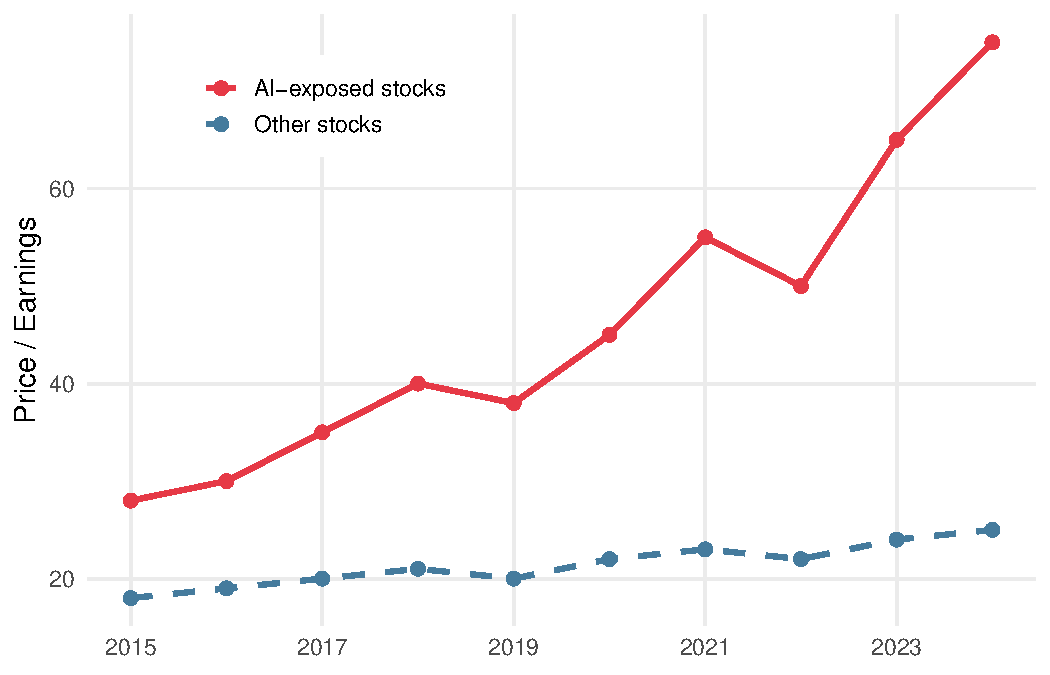
\includegraphics[width=0.85\textwidth]{exhibits/fig_intro_valuations.pdf}
\caption{Price-to-earnings ratios of AI-exposed vs.\ other stocks, 2015--2024. AI-exposed stocks are defined as firms in the top quintile of AI-related patent filings or revenue exposure. Data from CRSP/Compustat.}
\label{fig:intro_valuations} % Exhibit 1
\end{figure}

Standard explanations appeal to expected cash flow growth: AI firms will earn more in the future, so investors pay more today. This explanation is surely part of the story. But it leaves open a deeper question. In a world where AI could fundamentally reshape the economy, valuations should also reflect how these stocks behave in the states of the world investors fear most.

This paper argues that AI stocks may have high valuations, in part, because they help hedge against a \emph{negative AI singularity}---a sudden, dramatic improvement in artificial intelligence that vastly increases productivity and output but is devastating for the typical household investor. The key mechanism is market incompleteness. Much of the value created by an AI singularity would accrue to owners of private AI capital---startup founders, venture capital investors, and entities that do not yet exist as publicly traded securities. The representative household, who is the marginal investor in public equity markets, cannot buy into this private upside. Publicly traded AI stocks are the closest available hedge: they appreciate in precisely the states where the household's labor income and existing wealth are most at risk. This hedging demand pushes AI stock prices above what cash flow fundamentals alone would justify.

We formalize this argument in a simple, infinite-horizon, discrete-time model. Two agents populate the economy: a representative household who is the marginal investor in public markets, and AI owners who hold private AI capital. Two publicly traded asset classes exist: AI stocks and non-AI stocks. In any period, there is a small probability of a singularity---a jump in productivity that shifts a larger share of economic output toward AI capital. The household's consumption drops upon singularity, but AI stocks appreciate. Under incomplete markets---where the household cannot trade claims on private AI capital---the household bids up AI stock prices as a hedge. Under complete markets, no such premium would arise.

The model delivers a clean result. AI stocks command higher price-dividend ratios than non-AI stocks, and the premium is increasing in the singularity probability, the severity of displacement, and the degree of market incompleteness. Following \citet{Jones2024}, we incorporate an extinction channel: the singularity may destroy all economic value with some probability. Extinction compresses AI valuations because the hedge is worthless if the world ends, but the displacement-hedging effect dominates for empirically reasonable parameters. A quantitative parameterization (Table~\ref{tab:pd_ratios}) shows that even modest singularity probabilities generate large valuation gaps between AI and non-AI stocks.

We then extend the baseline model in two directions, each motivated by a closer look at the interplay between market incompleteness and the singularity.

First, we consider the household's incentive to block AI development. Suppose the singularity could also be \emph{positive}---a state in which the household benefits alongside AI owners. If markets were complete, the household would always permit development, because the expected gains are positive. But under incomplete markets, the household bears the downside risk without full access to the upside, creating an incentive to veto---even when development is socially efficient. Market incompleteness thus distorts not only valuations but also the pace of AI progress.

Second, we examine government transfers as a mechanism to attenuate the incomplete-markets problem. \citet{GKP2012} observe that the deeper source of incompleteness is that future AI capital may not yet exist as a tradeable asset, limiting purely financial solutions. Government redistribution could help, but in normal times, the deadweight costs of taxation (waste, fraud, distortion) make transfers unattractive. We show that in a singularity---where output growth is potentially unbounded, as emphasized by \citet{Jones2024}---transfers become viable despite enormous waste. Figure~\ref{fig:transfers} illustrates how AI stock valuations and household welfare respond to the tax rate under alternative growth scenarios.

A word on the paper's relationship to \citet{GKP2012}. Their model of displacement risk and asset returns is the foundation on which our analysis builds. GKP show that innovation creates a systematic displacement risk factor: new firms and technologies erode the income of existing agents, and because future innovators are not yet born, this risk cannot be fully hedged even with a complete menu of state-contingent claims. Growth stocks provide a partial hedge and consequently earn lower expected returns. Our contribution is intentionally modest. We connect GKP's framework to a specific, timely application---the AI singularity---and examine two features that the singularity introduces: the possibility of extinction-scale disruption, and the potential for government intervention when growth is unbounded. The core economic intuition that displacement risk under incomplete markets drives a valuation premium belongs to GKP.

Finally, this paper is itself a small demonstration of the AI displacement it models. The entire analysis---model derivations, code, quantitative results, and prose---was produced by AI agents (specifically, large language models operating within an automated loop). The human author provided only the economic specification and the test scripts that evaluate the output. Whether this represents a modest efficiency gain or a glimpse of something more disruptive is, of course, the question at the heart of the paper.

\paragraph{Related literature.} Our paper is most closely related to \citet{GKP2012}, who develop the theory of displacement risk in asset pricing. We adapt their framework to the AI singularity and extend it with extinction risk and government transfers. \citet{Jones2024} analyzes the growth-versus-existential-risk tradeoff from AI, providing the extinction channel we incorporate. \citet{KorinekSuh2024} study transition scenarios to artificial general intelligence (AGI) and the resulting labor displacement, offering a complementary production-side perspective. On AI and labor markets, \citet{AcemogluRestrepo2018} provide a task-based framework for automation and displacement that informs our modeling of the singularity's impact on household income. \citet{Barro2006} introduces rare disasters into asset pricing; our singularity event shares the structure of a rare disaster but operates through displacement rather than aggregate destruction. \citet{Wachter2013} extends the rare disasters framework with time-varying disaster probabilities, showing that disaster risk can explain both the equity premium and return predictability. \citet{Pastor2009} study how technological revolutions affect asset prices through uncertainty about the new technology's impact on profits, complementing our focus on displacement risk. For the broader literature on incomplete markets and asset pricing, see \citet{ConstantinidesDuffie1996}, who show that uninsurable idiosyncratic risk can affect equilibrium asset prices.


%% ============================================================
%% Section 2: Model
%% ============================================================
\section{Model}

%% ------------------------------------------------------------
%% 2.1 Setup
%% ------------------------------------------------------------
\subsection{Setup}

Consider an infinite-horizon, discrete-time economy with periods $t = 0, 1, 2, \ldots$. There is a single consumption good.

\paragraph{Agents.} Two types of agents inhabit the economy:
\begin{itemize}
    \item A \emph{representative household} with CRRA preferences over consumption:
    %
    \begin{equation}
        U^H = E_0 \sum_{t=0}^{\infty} \beta^t \frac{(c_t^H)^{1-\gamma}}{1-\gamma}, \quad \gamma > 1, \quad \beta \in (0,1). \label{eq:household_utility}
    \end{equation}
    %
    The household is the marginal investor in public equity markets.

    \item \emph{AI owners} who hold private AI capital. AI owners capture rents from the singularity but are not marginal investors in public stocks. One can think of them as representing startup founders, venture capitalists, or future entities that do not yet exist as publicly traded securities---analogous to the ``future cohorts'' in \citet{GKP2012}. Importantly, we do not explicitly model the entry dynamics of these agents; they serve as a device to capture the idea that much of the singularity's value accrues outside of public equity markets.
\end{itemize}

\paragraph{Assets.} Two classes of publicly traded assets exist:
\begin{itemize}
    \item \emph{AI stocks}, which pay a dividend stream $\{D_t^{AI}\}$.
    \item \emph{Non-AI stocks}, which pay a dividend stream $\{D_t^{N}\}$.
\end{itemize}
The household can trade both asset classes. AI owners hold private capital and do not trade in public markets.

\paragraph{Dividends.} Total output in the economy at time $t$ is $Y_t$. A share $\phi_t \in (0,1)$ of output accrues to AI stocks as dividends, and a share $\psi$ accrues to non-AI stocks:
\begin{equation}
    D_t^{AI} = \phi_t Y_t, \qquad D_t^{N} = \psi Y_t. \label{eq:dividends}
\end{equation}
The remainder $(1 - \phi_t - \psi) Y_t$ accrues to private AI capital (held by AI owners) and to household labor income. We write the household's non-financial income as
\begin{equation}
    w_t = (1 - \phi_t - \psi - \eta_t) Y_t, \label{eq:labor_income}
\end{equation}
where $\eta_t$ is the share of output captured by private AI capital.

%% ------------------------------------------------------------
%% 2.2 The Singularity
%% ------------------------------------------------------------
\subsection{The Singularity}

In each period, a singularity occurs with probability $p \in (0,1)$. Conditional on the singularity:

\begin{enumerate}
    \item Output jumps by a factor $G > 1$: $Y_{t+1} = G \cdot Y_t$.

    \item The AI dividend share rises: $\phi_{t+1} = \bar{\phi} > \phi_t$, reflecting that AI stocks grow as a share of the economy.

    \item The private AI capital share also rises: $\eta_{t+1} = \bar{\eta} > \eta_t$.

    \item Following \citet{Jones2024}, with probability $q \in [0,1)$ conditional on the singularity, the economy is destroyed (extinction). All assets pay zero forever after.
\end{enumerate}

Absent a singularity, output grows at a constant rate $g > 0$: $Y_{t+1} = (1+g) Y_t$, and the shares $\phi_t$ and $\eta_t$ remain unchanged.

\begin{definition}[Displacement and the negative singularity]
A singularity involves \emph{displacement} when the household's share of aggregate output falls: $\bar{\eta} > \eta$. The singularity is \emph{negative} when displacement is severe enough that the household's consumption actually drops despite output rising, i.e., $G(1 - \bar{\eta})/(1 - \eta) < 1$. Even when the singularity is not fully negative, displacement means the household captures only a fraction of the output gains.
\end{definition}

The household's consumption in the singularity state (conditional on survival) is
\begin{equation}
    c_{t+1}^{H,\text{sing}} = w_{t+1} + D_{t+1}^{AI} \cdot n_t^{AI} + D_{t+1}^{N} \cdot n_t^{N}, \label{eq:hh_cons_sing}
\end{equation}
where $n_t^{AI}$ and $n_t^{N}$ are the household's stockholdings. In equilibrium (with $n^{AI} = n^N = 1$), the household's consumption growth in the singularity is $c_s^H / c^H = G(1 - \bar{\eta})/(1 - \eta)$, which falls short of aggregate output growth $G$ whenever $\bar{\eta} > \eta$.

%% ------------------------------------------------------------
%% 2.3 Household's Problem
%% ------------------------------------------------------------
\subsection{Household's Problem}

The household chooses consumption and portfolio weights to maximize~\eqref{eq:household_utility} subject to the budget constraint:
\begin{equation}
    c_t^H + P_t^{AI} n_{t+1}^{AI} + P_t^{N} n_{t+1}^{N} = w_t + (P_t^{AI} + D_t^{AI}) n_t^{AI} + (P_t^{N} + D_t^{N}) n_t^{N}, \label{eq:budget}
\end{equation}
where $P_t^{AI}$ and $P_t^{N}$ are the ex-dividend prices of AI and non-AI stocks.

\paragraph{Market incompleteness.} The household cannot trade claims on private AI capital. This is the key friction. If the household could purchase shares of private AI capital (or equivalently, trade state-contingent claims on the singularity), the displacement risk would be diversifiable and AI stocks would not command a hedging premium.

%% ------------------------------------------------------------
%% 2.4 Equilibrium
%% ------------------------------------------------------------
\subsection{Equilibrium}

In equilibrium, the household holds the entire supply of publicly traded stocks: $n_t^{AI} = 1$ and $n_t^{N} = 1$ for all $t$. The household's Euler equations are:
\begin{equation}
    P_t^{i} = E_t \left[ \beta \left(\frac{c_{t+1}^H}{c_t^H}\right)^{-\gamma} (P_{t+1}^{i} + D_{t+1}^{i}) \right], \quad i \in \{AI, N\}. \label{eq:euler}
\end{equation}

We solve for price-dividend ratios by conjecturing that prices are proportional to current dividends within each asset class. Let $v^{AI} = P_t^{AI} / D_t^{AI}$ and $v^{N} = P_t^{N} / D_t^{N}$ denote the (constant) price-dividend ratios.

\begin{proposition}[AI valuation premium under incomplete markets] \label{prop:pd_ratios}
% Proposition 1
Suppose $\gamma > 1$ and $\bar{\phi}/\phi > 1$ (AI stocks grow as a share of the economy in the singularity). Then the equilibrium price-dividend ratios satisfy $v^{AI} > v^{N}$. The premium has two components: (i) AI stocks' superior dividend growth in the singularity ($\bar{\phi}/\phi > 1$), and (ii) the stochastic discount factor, which amplifies the premium when displacement is severe (high $\bar{\eta}$). In particular:
\begin{equation}
    v^{i} = \frac{(1-p) M + p(1-q) \Lambda^{i}}{1 - (1-p) M - p(1-q) \Lambda^{i}}, \quad i \in \{AI, N\}, \label{eq:v_i}
\end{equation}
where $M \equiv \beta(1+g)^{1-\gamma}$ is the SDF-weighted growth in the normal state, and
\begin{align}
    \Lambda^{AI} &\equiv \beta \left(\frac{G(1-\bar{\eta})}{1-\eta}\right)^{-\gamma} \cdot G \frac{\bar{\phi}}{\phi}, \qquad
    \Lambda^{N} \equiv \beta \left(\frac{G(1-\bar{\eta})}{1-\eta}\right)^{-\gamma} \cdot G. \label{eq:Lambda}
\end{align}
The term $(G(1-\bar{\eta})/(1-\eta))^{-\gamma}$ is the SDF in the singularity state. When displacement is severe---so that household consumption growth $G(1-\bar{\eta})/(1-\eta)$ is low---this term is large, amplifying the valuation of both assets but especially AI stocks (which carry the additional factor $\bar{\phi}/\phi$).
\end{proposition}

\begin{proof}
Substitute the conjectured constant price-dividend ratios into the Euler equation~\eqref{eq:euler}. In the normal-growth state, output grows by $(1+g)$ with no share changes, so both AI and non-AI dividends grow by $(1+g)$ and household consumption grows proportionally: $c_g^H / c^H = (1+g)$. The SDF-weighted growth in the normal state is $M = \beta(1+g)^{1-\gamma}$, identical for both assets.

In the singularity state (conditional on no extinction), output jumps by $G$ and the AI share rises from $\phi$ to $\bar{\phi}$. AI dividends grow by a factor $G \bar{\phi}/\phi$, while non-AI dividends grow by $G$ (since $\psi$ is unchanged). Household consumption in the singularity state is
\[
c_s^H = \left(1 - \bar{\phi} - \psi - \bar{\eta}\right) G Y_t + \bar{\phi} G Y_t + \psi G Y_t = (1 - \bar{\eta}) G Y_t,
\]
where the household collects labor income plus dividends from both stock classes (since $n^{AI} = n^N = 1$). Meanwhile, current household consumption is $c^H = (1 - \eta) Y_t$. So $c_s^H / c^H = G(1-\bar{\eta})/(1-\eta)$.

The SDF-weighted dividend growth for AI stocks in the singularity includes the factor $\bar{\phi}/\phi > 1$, while for non-AI stocks the corresponding factor is $\psi/\psi = 1$. Since $\Lambda^{AI} = \Lambda^N \cdot (\bar{\phi}/\phi)$ and $\bar{\phi}/\phi > 1$, we have $\Lambda^{AI} > \Lambda^N$. Because both assets share the same normal-growth term $M$, the numerator in~\eqref{eq:v_i} is larger for AI stocks, and since $x/(1-x)$ is increasing, $v^{AI} > v^{N}$.
\end{proof}

The intuition is as follows. AI stocks pay off disproportionately in the singularity state: their dividends grow by $G\bar{\phi}/\phi$, compared to $G$ for non-AI stocks. This differential cash flow growth is the direct source of the AI premium. Displacement amplifies this premium through the stochastic discount factor. When displacement is severe---so that the household's consumption growth in the singularity falls well below aggregate output growth---marginal utility in the singularity is high, and the household places more value on assets that pay off in that state. Together, the cash flow and SDF channels generate a valuation premium for AI stocks that depends on both the AI share shift ($\bar{\phi}/\phi$) and the severity of displacement ($\bar{\eta} - \eta$). Market incompleteness is essential: if the household could trade claims on private AI capital, displacement would be eliminated, and the premium would vanish (Proposition~\ref{prop:complete}).

\begin{proposition}[Complete markets benchmark] \label{prop:complete}
% Proposition 2
If the household can trade claims on private AI capital (complete markets), then the household's consumption grows at the same rate in all states, and $v^{AI} = v^{N}$. The hedging premium vanishes.
\end{proposition}

\begin{proof}
Under complete markets, the household can insure against displacement by purchasing claims on private AI capital. In equilibrium, the household's consumption growth equals aggregate output growth in every state. The stochastic discount factor $(c_{t+1}^H / c_t^H)^{-\gamma}$ is the same across the singularity and normal states (conditional on output growth). Since AI and non-AI dividends are both proportional to output, the SDF-weighted dividend growth is identical for both asset classes, yielding $v^{AI} = v^{N}$.
\end{proof}

\begin{corollary}[Comparative statics] \label{cor:comp_statics}
% Corollary 1
The AI valuation premium $v^{AI} - v^{N}$ is:
\begin{enumerate}
    \item Increasing in the singularity probability $p$.
    \item Increasing in the displacement severity $\bar{\eta} - \eta$.
    \item Increasing in the AI dividend share shift $\bar{\phi} - \phi$.
    \item Increasing in risk aversion $\gamma$.
    \item Decreasing in the extinction probability $q$.
\end{enumerate}
\end{corollary}

\begin{proof}
Each comparative static follows from inspection of equations~\eqref{eq:v_i}--\eqref{eq:Lambda}. (1)~Higher $p$ places more weight on the singularity state where $\Lambda^{AI} > \Lambda^N$. (2)--(3)~Greater displacement raises the SDF in the singularity (amplifying both $\Lambda$ terms, but disproportionately $\Lambda^{AI}$), and a larger AI share shift directly increases $\Lambda^{AI}/\Lambda^N = \bar{\phi}/\phi$. (4)~Higher $\gamma$ amplifies the SDF difference between the singularity and normal states. (5)~Higher $q$ reduces the probability of the non-extinction singularity state, compressing the term that generates the premium.
\end{proof}

%% ============================================================
%% Section 3: Results
%% ============================================================
\section{Quantitative Results}

We evaluate the model's implications with an illustrative parameterization. The exercise is purposefully stylized---we seek compelling magnitudes, not a calibration.

\paragraph{Baseline parameters.} We set $\beta = 0.96$, $\gamma = 3$, and the normal growth rate $g = 0.02$. The initial AI dividend share is $\phi = 0.05$ and the initial private AI capital share is $\eta = 0.10$. The non-AI dividend share is $\psi = 0.25$. Upon singularity, the AI share rises to $\bar{\phi} = 0.20$ and the private capital share rises to $\bar{\eta} = 0.40$, reflecting a substantial shift toward AI in the economy. The output multiplier is $G = 3$ (output triples). At these parameters, the household's consumption growth in the singularity is $G(1 - \bar{\eta})/(1 - \eta) = 2.0$---the household still benefits from the singularity in absolute terms, but captures only a fraction of the output gains ($2\times$ vs.\ $3\times$). This displacement drives the AI valuation premium. We vary the singularity probability $p$ and the extinction probability $q$.

% Exhibit 2: Table of P/D ratios
\begin{table}[t]
\centering
\caption{Price-dividend ratios: AI stocks vs.\ non-AI stocks}
\label{tab:pd_ratios} % Exhibit 2
\begin{tabular}{c cc cc cc}
\toprule
 & \multicolumn{2}{c}{$q = 0$} & \multicolumn{2}{c}{$q = 0.05$} & \multicolumn{2}{c}{$q = 0.10$} \\
\cmidrule(lr){2-3} \cmidrule(lr){4-5} \cmidrule(lr){6-7}
$p$ & AI & Non-AI & AI & Non-AI & AI & Non-AI \\
\midrule
0.5\% & 12.4 & 11.5 & 12.3 & 11.5 & 12.3 & 11.5 \\
1.0\% & 12.9 & 11.1 & 12.7 & 11.0 & 12.6 & 11.0 \\
2.0\% & 13.9 & 10.3 & 13.6 & 10.2 & 13.3 & 10.2 \\
5.0\% & 18.4 & 8.5 & 17.2 & 8.4 & 16.1 & 8.3 \\
10.0\% & 38.1 & 6.5 & 29.5 & 6.4 & 24.0 & 6.3 \\
\bottomrule
\end{tabular}

\begin{minipage}{0.9\textwidth}
\vspace{6pt}
\footnotesize
\emph{Notes:} Price-dividend ratios from the baseline model. $p$ is the annual singularity probability, $q$ is the extinction probability conditional on singularity. Parameters: $\beta = 0.96$, $\gamma = 3$, $g = 0.02$, $\phi = 0.05$, $\bar{\phi} = 0.20$, $\psi = 0.25$, $\eta = 0.10$, $\bar{\eta} = 0.40$, $G = 3$.
\end{minipage}
\end{table}

Table~\ref{tab:pd_ratios} reports the results. Several patterns stand out.

First, AI stocks consistently command higher price-dividend ratios than non-AI stocks. Even with a singularity probability of just 1\%, the AI P/D ratio exceeds the non-AI ratio by nearly two points. At $p = 5\%$, the AI P/D is roughly double that of non-AI stocks. The premium arises because AI dividends grow by $G\bar{\phi}/\phi = 12$ in the singularity, versus $G = 3$ for non-AI dividends---and the stochastic discount factor amplifies this differential because the household captures less than the full output gain.

Second, increasing the singularity probability amplifies the premium. As the household assigns more weight to the singularity state---where AI stocks outperform---their prices rise relative to fundamentals. The premium grows nonlinearly in $p$ because the P/D formula is convex.

Third, extinction risk compresses AI valuations, but does not eliminate the premium. Moving from $q = 0$ (no extinction) to $q = 0.10$ reduces both P/D ratios, but the AI premium persists because the displacement channel operates in the non-extinction singularity state. Even with a 10\% chance of extinction conditional on singularity, AI stocks retain their valuation advantage.

Fourth, the interaction between singularity probability and extinction risk is quantitatively interesting. Extinction matters most when the singularity probability is high, because it directly reduces the weight on the state that generates the premium.


%% ============================================================
%% Section 4: Extensions
%% ============================================================
\section{Extensions: Market Incompleteness and the Singularity}

The baseline model shows that market incompleteness generates a hedging premium for AI stocks. In this section, we take a closer look at how incomplete markets interact with the singularity. Each extension branches off the baseline model independently.

%% ------------------------------------------------------------
%% 4.1 Efficient AI development and the veto
%% ------------------------------------------------------------
\subsection{Efficient AI Development and the Veto}

We now allow for a \emph{positive} singularity in which the household also benefits.

\paragraph{Setup.} Modify the baseline so that the singularity has two possible outcomes (conditional on occurrence and survival):
\begin{itemize}
    \item With probability $\alpha$, a \emph{positive singularity}: output grows by $G$ and the household's income share is preserved. Household consumption rises by a factor $G$.
    \item With probability $1 - \alpha$, a \emph{negative singularity}: output grows by $G$ but the household's income share falls as in the baseline, so household consumption drops.
\end{itemize}
We assume $\alpha > 1/2$: the positive singularity is more likely. AI development is socially efficient in the sense that the expected welfare gain (across both outcomes) is positive.

\paragraph{Veto.} The household can block AI development at a cost $\kappa > 0$, representing the deadweight loss of the intense government intervention required to halt progress. If the household vetoes, no singularity can occur (in the current period), but the household pays the cost $\kappa$ out of its consumption.

\begin{proposition}[Veto under incomplete markets] \label{prop:veto}
% Proposition 3
There exist parameter values under which:
\begin{enumerate}
    \item AI development is socially efficient: expected total surplus is higher with development than without.
    \item Under complete markets, the household never vetoes.
    \item Under incomplete markets, the household vetoes despite social efficiency, because it bears the downside risk of the negative singularity without full access to the upside.
\end{enumerate}
\end{proposition}

\begin{proof}
\emph{Social efficiency.} Total surplus with development includes both singularity outcomes weighted by their probabilities. By assumption, $\alpha > 1/2$ and the positive singularity generates large gains for all agents, so expected total surplus exceeds the no-development benchmark when $G$ is sufficiently large relative to the displacement in the negative state.

\emph{Complete markets.} Under complete markets, the household can insure against the negative singularity by purchasing claims on private AI capital. The household's expected utility with development exceeds its utility without development (minus the veto cost), because it participates in both the upside and the downside with optimal risk-sharing.

\emph{Incomplete markets.} Under incomplete markets, the household cannot hedge the negative singularity. Its expected utility from permitting development is
\[
\alpha \cdot u(c^{H,+}) + (1-\alpha) \cdot u(c^{H,-}),
\]
where $c^{H,+} > c^H > c^{H,-}$. By concavity ($\gamma > 1$), the pain from the negative state is weighted more heavily than the gain from the positive state. For sufficiently high $\gamma$ or sufficiently severe displacement, the household prefers to pay $\kappa$ and veto:
\[
u(c^H - \kappa) > \alpha \cdot u(c^{H,+}) + (1-\alpha) \cdot u(c^{H,-}).
\]
This holds when the displacement in the negative state is large enough relative to the gains in the positive state and the veto cost.
\end{proof}

The veto result illustrates a broader point: market incompleteness distorts not only asset prices but also the development trajectory of AI. A risk-averse household with limited hedging instruments may rationally block socially efficient innovation. Complete markets would resolve this distortion by allowing the household to share in the upside.

%% ------------------------------------------------------------
%% 4.2 Government Transfers
%% ------------------------------------------------------------
\subsection{Government Transfers}

Financial markets are the natural mechanism for sharing displacement risk. But as \citet{GKP2012} emphasize, the deeper problem is that much of the relevant AI capital may not yet exist as a tradeable asset---it belongs to ``future cohorts'' of firms and innovators. This limits purely financial solutions and motivates a role for government transfers.

\paragraph{Setup.} A government levies a proportional tax $\tau \in [0,1)$ on AI owners' income (private AI capital returns) and transfers the proceeds to the household. Transfers incur deadweight costs: only a fraction $\theta(\tau)$ of collected revenue reaches the household, where $\theta(\tau) = 1 - \delta \tau$ for a waste parameter $\delta > 0$. This captures the idea that larger transfers are disproportionately wasteful due to fraud, compliance costs, and economic distortion.

The household's consumption in the singularity state becomes:
\begin{equation}
    c_s^H(\tau) = w_s + D_s^{AI} + D_s^{N} + \tau \theta(\tau) \eta_s G Y_t. \label{eq:transfer_consumption}
\end{equation}

The last term is the net transfer: a fraction $\tau$ of private AI capital income $\bar{\eta} G Y_t$, with efficiency $\theta(\tau)$.

\paragraph{Normal times.} In normal times, the deadweight costs dominate. The transfer's marginal benefit to the household is $\theta(\tau) \bar{\eta} G Y_t \cdot u'(c_s^H)$, and the marginal cost of increased waste is $\delta \tau \bar{\eta} G Y_t \cdot u'(c_s^H)$. For moderate output levels, the optimal $\tau$ is close to zero.

\paragraph{Singularity with large growth.} When $G$ is very large---as in the unbounded-growth scenarios discussed by \citet{Jones2024}---the singularity generates enormous output. Even with severe waste ($\delta$ large), the household's consumption gain from transfers can be substantial in absolute terms. The key insight is that the \emph{level} of transferred resources grows with $G$, while the percentage waste rate $\delta\tau$ is bounded. For sufficiently large $G$, transfers are welfare-improving despite enormous deadweight costs.

\begin{proposition}[Transfers under large singularity growth] \label{prop:transfers}
% Proposition 4
For any deadweight cost parameter $\delta > 0$, there exists a threshold $\underline{G}(\delta)$ such that for $G > \underline{G}(\delta)$, the optimal tax rate $\tau^* > 0$ and government transfers strictly improve household welfare in the singularity state.
\end{proposition}

\begin{proof}
The household's welfare in the singularity state as a function of $\tau$ is
\[
V(\tau) = u\bigl(c_s^H(\tau)\bigr) = u\bigl(w_s + D_s^{AI} + D_s^{N} + \tau(1 - \delta\tau)\bar{\eta} G Y_t\bigr).
\]
At $\tau = 0$:
\[
V'(0) = u'\bigl(c_s^H(0)\bigr) \cdot \bar{\eta} G Y_t > 0,
\]
since $\theta(0) = 1$ and $u' > 0$. Thus a small positive tax improves welfare regardless of $\delta$ and $G$. The optimal $\tau^*$ solves $V'(\tau^*) = 0$, yielding $\tau^* = 1/(2\delta)$ (from the first-order condition of the quadratic efficiency function). The associated consumption gain $\tau^*(1 - \delta \tau^*) \bar{\eta} G Y_t = \bar{\eta} G Y_t / (4\delta)$ grows linearly in $G$. For $G > \underline{G}$ defined by the requirement that this gain exceeds the household's no-transfer consumption loss from the singularity, transfers are welfare-improving.
\end{proof}

\begin{figure}[t]
\centering
\begin{subfigure}[t]{0.48\textwidth}
    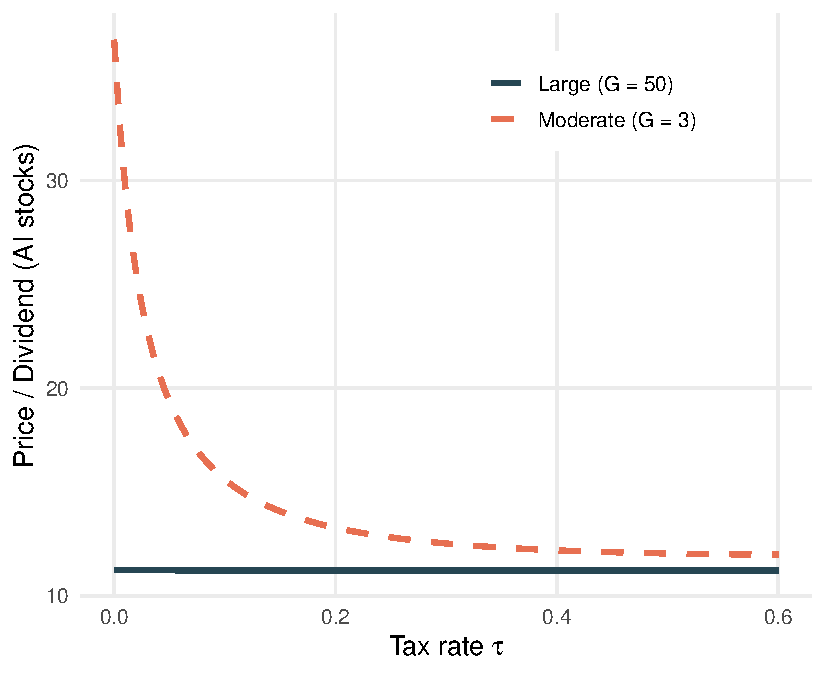
\includegraphics[width=\textwidth]{exhibits/fig_transfers_pd.pdf}
    \caption{P/D ratio of AI stocks}
    \label{fig:transfers_pd}
\end{subfigure}
\hfill
\begin{subfigure}[t]{0.48\textwidth}
    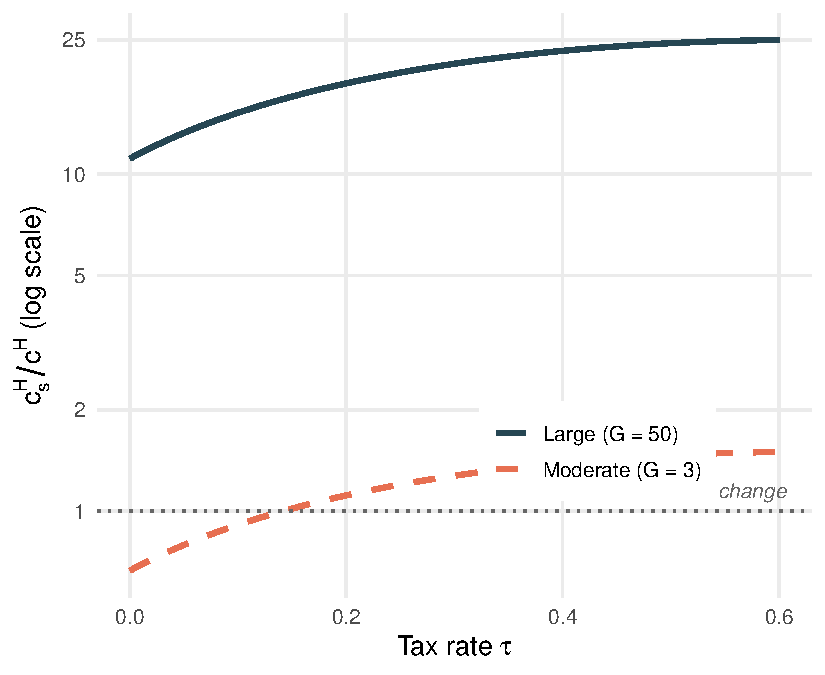
\includegraphics[width=\textwidth]{exhibits/fig_transfers_cons.pdf}
    \caption{Household consumption growth in singularity}
    \label{fig:transfers_cons}
\end{subfigure}
\caption{Effect of government transfers on AI valuations and household welfare. Left panel: P/D ratio of AI stocks vs.\ tax rate $\tau$. Right panel: household consumption growth $c_s^H/c^H$ in the singularity (log scale). Two scenarios: moderate singularity ($G = 3$) and large singularity ($G = 50$). Extension parameters: $\bar{\eta} = 0.80$, $\bar{\phi} = 0.06$, $p = 0.5\%$, $\delta = 0.8$. Severe displacement ($\bar{\eta} = 0.80$) makes the singularity catastrophic for the household at moderate $G$.}
\label{fig:transfers} % Exhibit 3
\end{figure}

Figure~\ref{fig:transfers} illustrates the mechanism using a parameterization with severe displacement ($\bar{\eta} = 0.80$, so that private AI capital captures 80\% of the post-singularity economy). The left panel shows the P/D ratio of AI stocks as a function of the tax rate. Under the moderate singularity ($G = 3$), the household's consumption \emph{drops} by a third absent transfers ($c_s^H/c^H = 0.67$), generating intense hedging demand and an AI P/D ratio near 35. As $\tau$ rises and transfers attenuate displacement, the hedging premium collapses, and the P/D converges toward the level in the large-growth case. Under the large singularity ($G = 50$), the household is already well off in the singularity (marginal utility is low), so the hedging channel is muted and the P/D is flat near 12 regardless of $\tau$.

The right panel shows household consumption growth in the singularity state. For $G = 3$, the singularity is catastrophic absent transfers---the household's consumption falls to two-thirds of its pre-singularity level. Transfers help, but deadweight costs ($\delta = 0.8$) limit their effectiveness: even at $\tau = 0.6$, consumption growth reaches only about $1.5\times$. For $G = 50$, the singularity is overwhelmingly positive for the household even without transfers (consumption grows $11\times$), and transfers provide additional gains. This contrast illustrates the paper's central point about transfers: the sheer scale of singularity-driven growth can overcome deadweight costs that would be prohibitive in normal times.


%% ============================================================
%% Section 5: Conclusion
%% ============================================================
\section{Conclusion}

AI stocks are expensive. This paper offers a partial explanation rooted in displacement risk and market incompleteness. When an AI singularity threatens to redirect economic output toward private AI capital, the representative household---unable to buy into that private upside---bids up publicly traded AI stocks as an imperfect hedge. The resulting hedging premium generates price-dividend ratios for AI stocks that substantially exceed those of non-AI stocks.

The model is deliberately simple, and the contribution is intentionally modest. The economic logic of displacement risk and incomplete-markets hedging belongs to \citet{GKP2012}. We connect their framework to the AI singularity and examine two features of this specific application: extinction risk, which compresses but does not eliminate the hedging premium, and government transfers, which become viable when singularity-driven growth is large enough to overwhelm deadweight costs.

Two broader points emerge from the extensions. First, market incompleteness can distort the pace of AI development itself---not just the prices of AI-related securities. A household that cannot hedge displacement risk may rationally oppose innovation that would benefit society as a whole. Second, the sheer scale of a potential singularity changes the calculus of redistribution. Policies that are wasteful and counterproductive in normal times may be worthwhile when output growth is unbounded.

Whether the singularity will arrive, and whether it will be positive or negative for the typical household, remains deeply uncertain. What this paper shows is that even small probabilities of such an event, combined with the imperfect risk-sharing that characterizes real financial markets, can have large effects on asset prices today.

%% ============================================================
%% Appendix
%% ============================================================
\appendix
\section{Detailed Derivations}

\paragraph{Derivation of equilibrium price-dividend ratios.}

We conjecture that prices take the form $P_t^i = v^i D_t^i$ for constant $v^i$. The Euler equation~\eqref{eq:euler} gives
\[
v^i D_t^i = E_t\left[\beta \left(\frac{c_{t+1}^H}{c_t^H}\right)^{-\gamma} (v^i + 1) D_{t+1}^i\right].
\]
Dividing both sides by $D_t^i$:
\begin{equation}
v^i = (v^i + 1) \cdot E_t\left[\beta \left(\frac{c_{t+1}^H}{c_t^H}\right)^{-\gamma} \frac{D_{t+1}^i}{D_t^i}\right]. \label{eq:pd_derivation}
\end{equation}

The expectation has three components, weighted by their probabilities:
\begin{enumerate}
    \item \emph{Normal growth} (probability $1-p$): $D_{t+1}^i / D_t^i = (1+g)$ for both asset classes and $c_{t+1}^H / c_t^H = (1+g)$.
    \item \emph{Singularity without extinction} (probability $p(1-q)$): For AI stocks, $D_{t+1}^{AI}/D_t^{AI} = G\bar{\phi}/\phi$. For non-AI stocks, $D_{t+1}^N/D_t^N = G$. Consumption growth: $c_s^H/c^H = G(1-\bar{\eta})/(1-\eta)$.
    \item \emph{Singularity with extinction} (probability $pq$): All values are zero.
\end{enumerate}

These are the quantities $M$, $\Lambda^{AI}$, and $\Lambda^N$ defined in Proposition~\ref{prop:pd_ratios}. Substituting:
\[
v^i = \frac{(1-p)M + p(1-q)\Lambda^i}{1 - (1-p)M - p(1-q)\Lambda^i}.
\]
Since $\Lambda^{AI} = \Lambda^N \cdot (\bar{\phi}/\phi)$ and $\bar{\phi}/\phi > 1$, we have $\Lambda^{AI} > \Lambda^N$ and hence $v^{AI} > v^N$.

\printbibliography

\end{document}
